\documentclass{article}
\usepackage[utf8]{inputenc}
\usepackage[greek,english]{babel} \usepackage{alphabeta}
\usepackage{fancyhdr}
\usepackage{listings}
\usepackage{mathtools}
\usepackage{xcolor}
\usepackage{graphicx}
\usepackage{float}
\usepackage[backend=biber]{biblatex}

\title{Σήματα και Συστήματα - Εργασία 2}
\author{Χρήστος Μαργιώλης - 19390133}
\date{Απρίλιος 2021}

\begin{document}

\begin{titlepage}
        \maketitle
        \begin{figure}[t!]
        \begin{center}
        
\includegraphics[scale=0.3]{./res/uniwalogo.png} \\
        \Large
        \textbf{Πανεπιστήμιο Δυτικής Αττικής} \\
        \large
        Τμήμα Μηχανικών Πληροφορικής και Ηλεκτρονικών Υπολογιστών
        \end{center}
        \end{figure}
\end{titlepage}

\renewcommand{\contentsname}{Περιεχόμενα}
\tableofcontents

\section{'Ασκηση 1}

\begin{itemize}
        \item Να σχεδιαστεί το σήμα
                \[x(t) = u(t + 1) - u(t - 2) + u(t + 4)\]
\end{itemize}

Αρχικά ορίζουμε ένα χρονικό διάστημα $t$ - θα το ορίσουμε από το -5 εώς το 10:
\begin{lstlisting}[language=octave]
        octave> t = -5:0.1:10
\end{lstlisting}

Με τη χρήση της συνάρτησης \lstinline{heaviside()} θα υπολογίσουμε τις
τιμές των συναρτήσεων $u(t + 1)$, $u(t - 2)$ και $u(t + 4)$. Μπορούμε
για κάθε συνάρτηση να αποθηκεύσουμε την έξοδό της \lstinline{heaviside()}
σε μία προσωρινή μεταβλητή, αλλά για μεγαλύτερη άνεση και εξοικονόμιση
χρόνου θα αποθηκεύσουμε τα πάντα κατευθείαν στο $x$:
\begin{lstlisting}[language=octave]
        octave> x = heaviside(t+1)-heaviside(t-2)+heaviside(t+4)
\end{lstlisting}

Τέλος, σχεδιάζουμε το σήμα $x(t)$ και τροποποιούμε τον άξονα $x$
για καλύτερη εμφάνιση της γραφικής παράστασης:
\begin{lstlisting}[language=octave]
        octave> plot(t, x)
        octave> xlim([-5 10])
\end{lstlisting}

\begin{figure}[H]
        \centering
        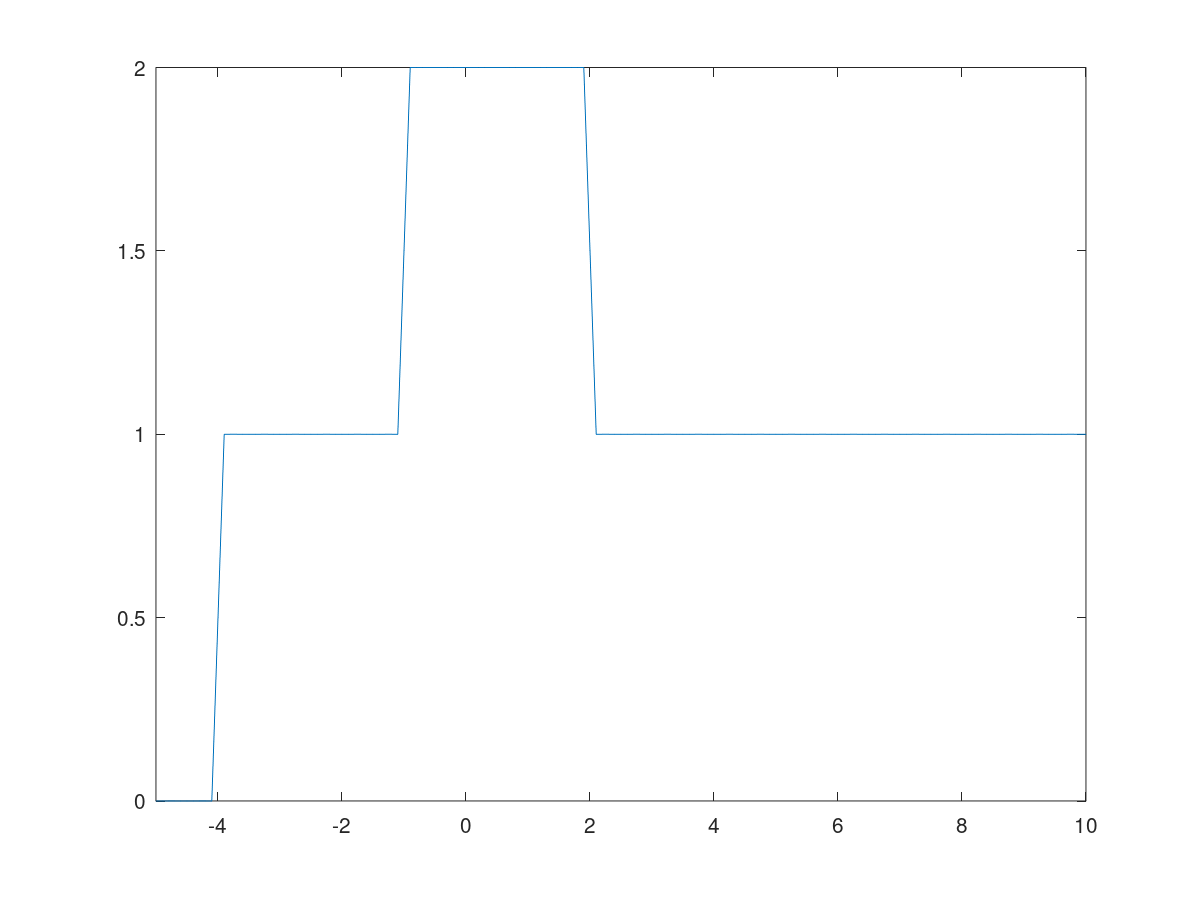
\includegraphics[width=\linewidth]{res/fig2.png}
        \caption{$x(t) = u(t + 1) - u(t - 2) + u(t + 4)$ με τη χρήση της
                \lstinline{heaviside()}}
\end{figure}

\section{'Ασκηση 2}

\begin{itemize}
        \item Να σχεδιαστεί το σήμα
                \[x(t) = t\sin(2\pi t)(u(t) - u(t - 3))\]
\end{itemize}

Αρχικά ορίζουμε το διάστημα το χρονικό διάστημα $t$ από από το -5 ως το 10:
\begin{lstlisting}[language=octave]
        octave> t = -5:0.1:10
\end{lstlisting}

Για να υπολογίσουμε τις τιμές των μοναδιαίων βηματικών συναρτήσεων $u(t)$
και $u(t - 3)$ θα χρησιμοποιήσουμε κατευθείαν την συνάρτηση 
\lstinline{heaviside()}:
\begin{lstlisting}[language=octave]
        octave> x = t.*sin(2*pi*t).*(heaviside(t)-heaviside(t-3))
\end{lstlisting}

Τέλος, σχεδιάζουμε το σήμα $x(t)$ και τροποποιούμε τον άξονα $x$
για καλύτερη εμφάνιση της γραφικής παράστασης:
\begin{lstlisting}[language=octave]
        octave> plot(t, x)
        octave> xlim([-5 10])
\end{lstlisting}

\begin{figure}[H]
        \centering
        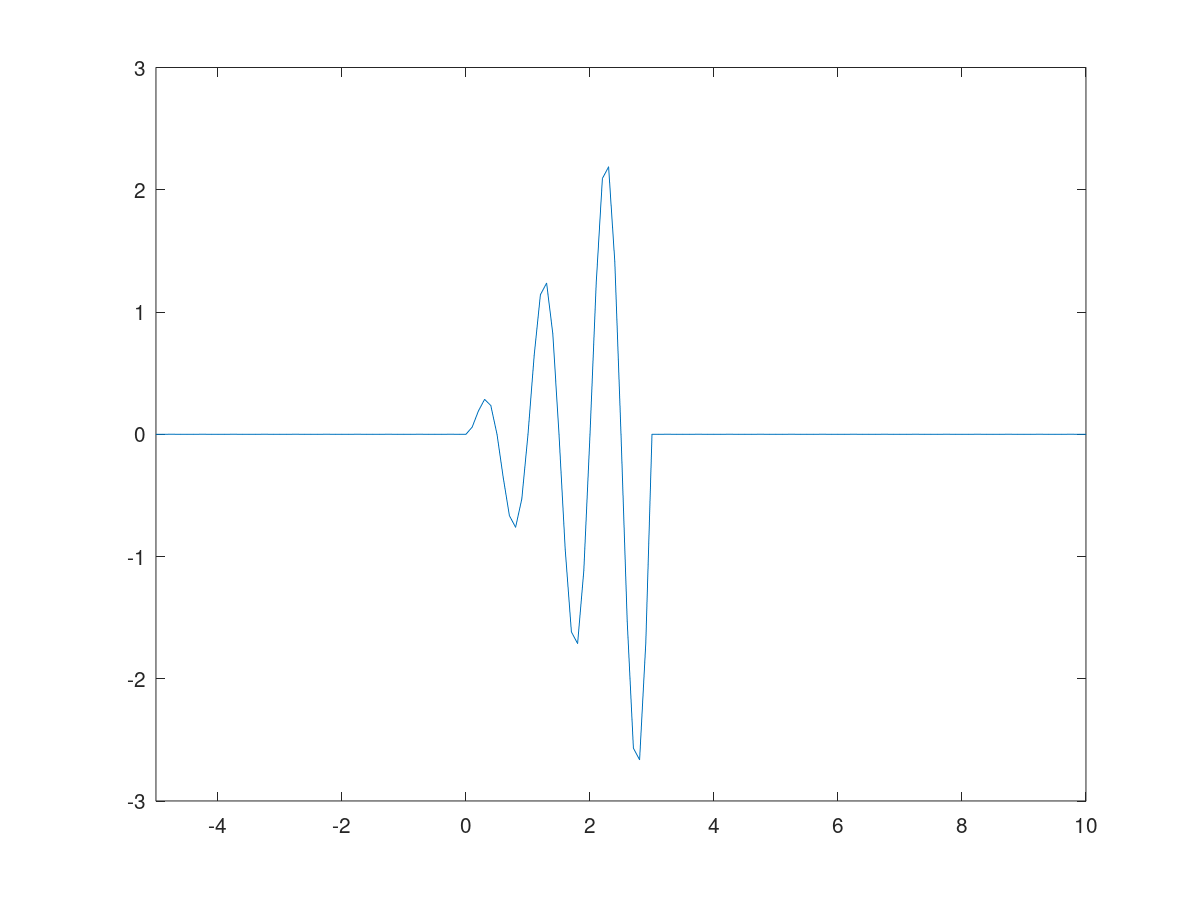
\includegraphics[width=\linewidth]{res/fig3.png}
        \caption{$x(t) = t\sin(2\pi t)(u(t) - u(t - 3))$}
\end{figure}

\section{'Ασκηση 3}

\begin{itemize}
        \item Να σχεδιαστεί το σήμα
                \[x(t) = t^3 \cos(10\pi t)p 2(t - 1)\]
                όπου $pT(t)$ τετραγωνικός παλμός διάρκειας $T$.
\end{itemize}

Ο τετραγωνικός παλμός $pT(t)$ ορίζεται ως
\[pT(t) = u(t + \frac{T}{2}) - u(t - \frac{T}{2})\]
Οπότε, με βάση την εκφώνηση και τον παραπάνω τύπο έχουμε ότι:
\[p2(t - 1) \Rightarrow u(t - 1 + \frac{2}{2}) - u(t - 1 - \frac{2}{2})
\Rightarrow u(t - 1 + 1) - u(t - 1 - 1) \Rightarrow u(t) - u(t - 2)\]

Τώρα, με την χρήση της συνάρτησης \lstinline{heaviside()} μπορούμε να
υπολογίσουμε τις τιμές του τετραγωνικού παλμού $p2(t - 1)$:
\begin{lstlisting}[language=octave]
        octave> p = heaviside(t)-heaviside(t-2)
\end{lstlisting}

'Εχοντας το $p2(t - 1)$ μπορούμε τώρα να υπολογίσουμε και να σχεδιάσουμε
το σήμα $x(t)$. Επίσης θα τροποποιήσουμε τον άξονα $x$ ώστε να εμφανιστεί
πιο καθαρά η γραφική παράσταση:
\begin{lstlisting}[language=octave]
        octave> x = t.^3.*cos(10*pi*t).*p
        octave> plot(t, x)
        octave> xlim([-5 10])
\end{lstlisting}

\begin{figure}[H]
        \centering
        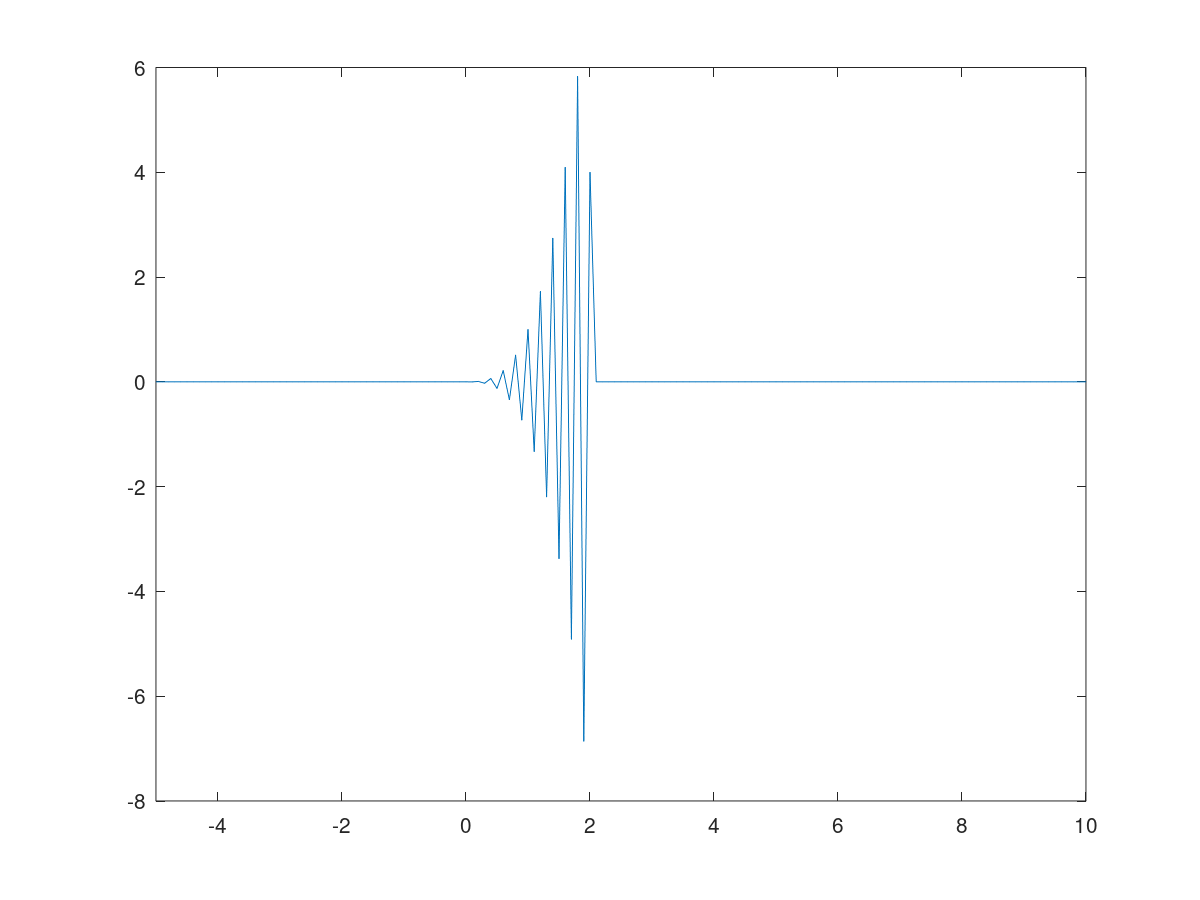
\includegraphics[width=\linewidth]{res/fig4.png}
        \caption{$x(t) = t^3cos(10\pi t)p2(t - 1)$}
\end{figure}

\section{'Ασκηση 4}

\begin{itemize}
        \item Να εκφταστεί και να σχεδιαστεί το σήμα (φυλλάδιο εργασίας
                σελίδα 28) ως άθροισμα μόνο συναρτήσεων ράμπας.
\end{itemize}

Η συνάρτηση ράμπας ορίζεται ως:
\[r(t) = tu(t)\]
Στο Octave, αυτό υπολογίζεται ως:
\begin{lstlisting}[language=octave]
        octave> r = t.*heaviside(t)
\end{lstlisting}
Οπότε θα φτιάξουμε μία συνάρτηση - θα την ονομάσουμε \lstinline{ramp} -
η οποία θα υπολογίζει την συνάρτηση ράμπας. Η συνάρτηση θα δέχεται
ως όρισμα ένα $t$ και θα επιστρέφει τις τιμές της συνάρτησης $r(t)$:
\begin{lstlisting}[language=octave]
        function r = ramp(t)
                r = t.*heaviside(t)
        endfunction
\end{lstlisting}

Το σήμα που ζητάει η εκφώνηση εκφράζεται ως
\[x(t) = r(t) - r(t-1) - r(t-2)\]
και το χρονικό διάστημα είναι το $t = [-2,3]$. Οπότε:
\begin{lstlisting}[language=octave]
        octave> t = -2:0.1:3
        octave> r = ramp(t)-ramp(t-1)-ramp(t-2)
        octave> plot(t, r)
        octave> ylim([-0.3 1.3])
\end{lstlisting}

\begin{figure}[H]
        \centering
        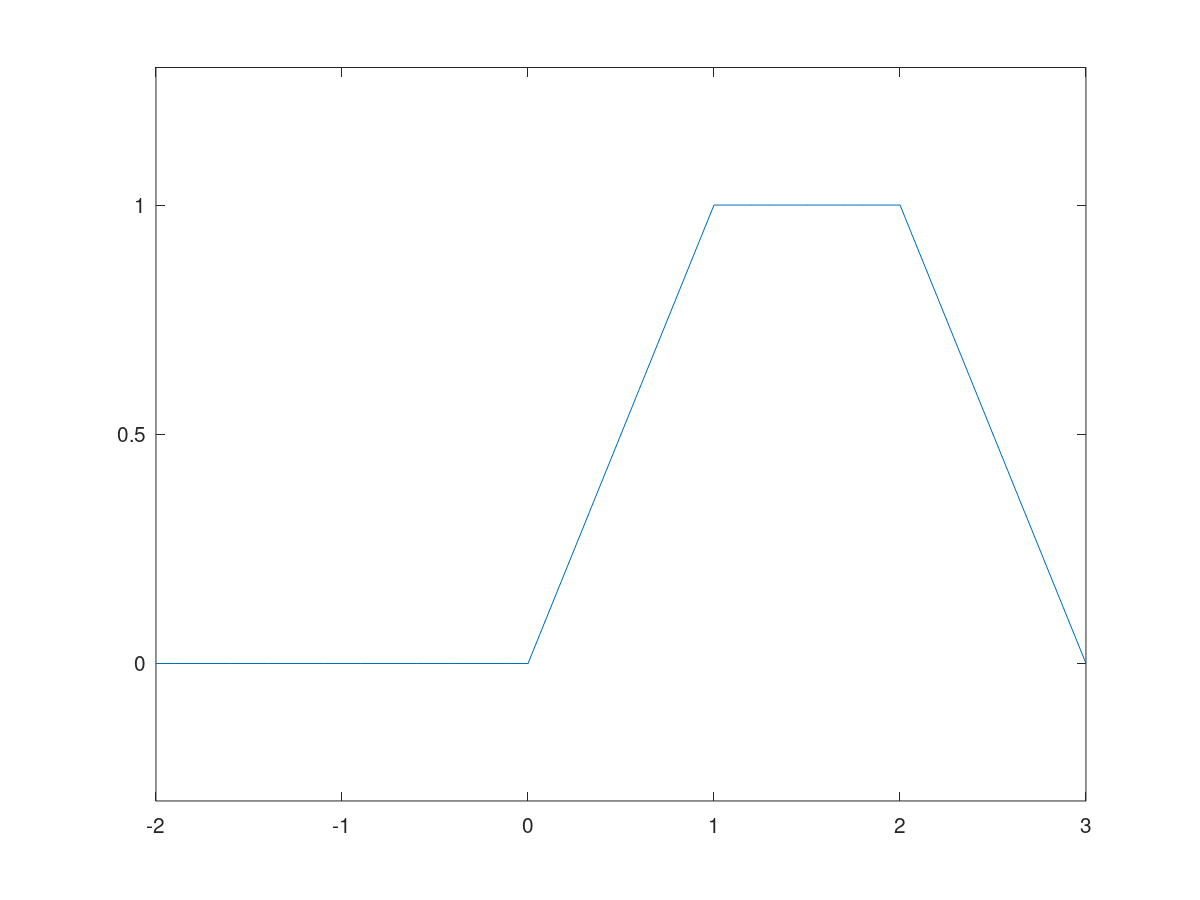
\includegraphics[width=\linewidth]{res/fig7.png}
        \caption{$x(t) = r(t) - r(t-1) - r(t-2)$}
\end{figure}

\section{'Ασκηση 5}

\begin{itemize}
        \item Δίνεται το σήμα
                \[x(t) = te^{-t}, 0 \leq t \leq 5\]
                Να σχεδιαστούν:
        \begin{itemize}
                \item Το σήμα $x(t)$
                \item Το άρτιο σήμα $x_e(t)$ του $x(t)$
                \item Το περιττό σήμα $x_o(t)$ του $x(t)$
                \item Το άθροισμα $x_e(t) + x_o(t)$
        \end{itemize}
\end{itemize}

Θα σχεδιάσουμε τα τέσσερα ζητούμενα σήματα στο ίδιο παράθυρο με την
χρήση της συνάρτησης \lstinline{subplot()}.

Αρχικά ορίζουμε το διάστημα $t = [0, 5]$:
\begin{lstlisting}[language=octave]
        octave> t = 0:0.1:5
\end{lstlisting}

Υπολογίζουμε τις τιμές του σήματος $x(t) = te^{-t}$ και σχεδιάζουμε το σήμα.
Σε όλα τα σήματα που θα σχεδιάσουμε θα τους δώσουμε και επίσης και έναν τίτλο
ώστε να μπορούμε να ξεχωρίσουμε σε ποιο σήμα αντιστοιχεί η κάθε γραφική
παράσταση:
\begin{lstlisting}[language=octave]
        octave> x = t.*exp(-t)
        octave> sublot(2, 2, 1)
        octave> plot(t, x)
        octave> title("x(t) = t.*exp(-t)")
\end{lstlisting}

Το άρτιο μέρος ενός σήματος ορίζεται ως:
\[x_e(t) = \frac{1}{2}(x(t) + x(-t))\]
και το περιττό μέρος ως:
\[x_o(t) = \frac{1}{2}(x(t) - x(t))\]
Για να υπολογίσουμε το $x(-t)$ θα μπορούσαμε να φτιάξουμε μία νέα μεταβλητή
$-t$ η οποία θα κρατάει το διάστημα χρόνου αντιστραμένο - δηλαδή
$-t = [-5, 0]$ - αλλά το Octave παρέχει την συνάρτηση \lstinline{fliplr()}
η οποία μπορεί να αντιστρέψει ένα διάνυσμα. Το αποτέλεσμα της
\lstinline{fliplr()} θα το αποθηκεύσουμε στο διάνυσμα \lstinline{xrev}
ώστε να το χρησιμοποιήσουμε για τον υπολογισμό του αρτίου και περιττού
σήματος:
\begin{lstlisting}[language=octave]
        octave> xrev = fliplr(x)
        octave> xe = 0.5*(x + xrev)
        octave> xo = 0.5*(x - xrev)
        octave> subplot(2, 2, 2)
        octave> plot(t, xe)
        octave> title("x_{even}")
        octave> subplot(2, 2, 3)
        octave> plot(t, xo)
        octave> title("x_{odd}")
\end{lstlisting}

Για τον υπολογισμό του αθροίσματος, απλώς προσθέτουμε τα σήματα
$x_e(t)$ και $x_o(t)$ που υπολογίσαμε παραπάνω.
\begin{lstlisting}[language=octave]
        octave> xeo = xe + xo
        octave> subplot(2, 2, 4)
        octave> plot(t, xeo)
        octave> title("x_{eo}")
\end{lstlisting}

Παρατηρούμε ότι ισχύει
\[x(t) = x_e + x_o\]
δηλαδή το άθροισμα του αρτίου και του περιττού σήματος είναι ίσο
με το αρχικό σήμα $x(t)$:
\begin{figure}[H]
        \centering
        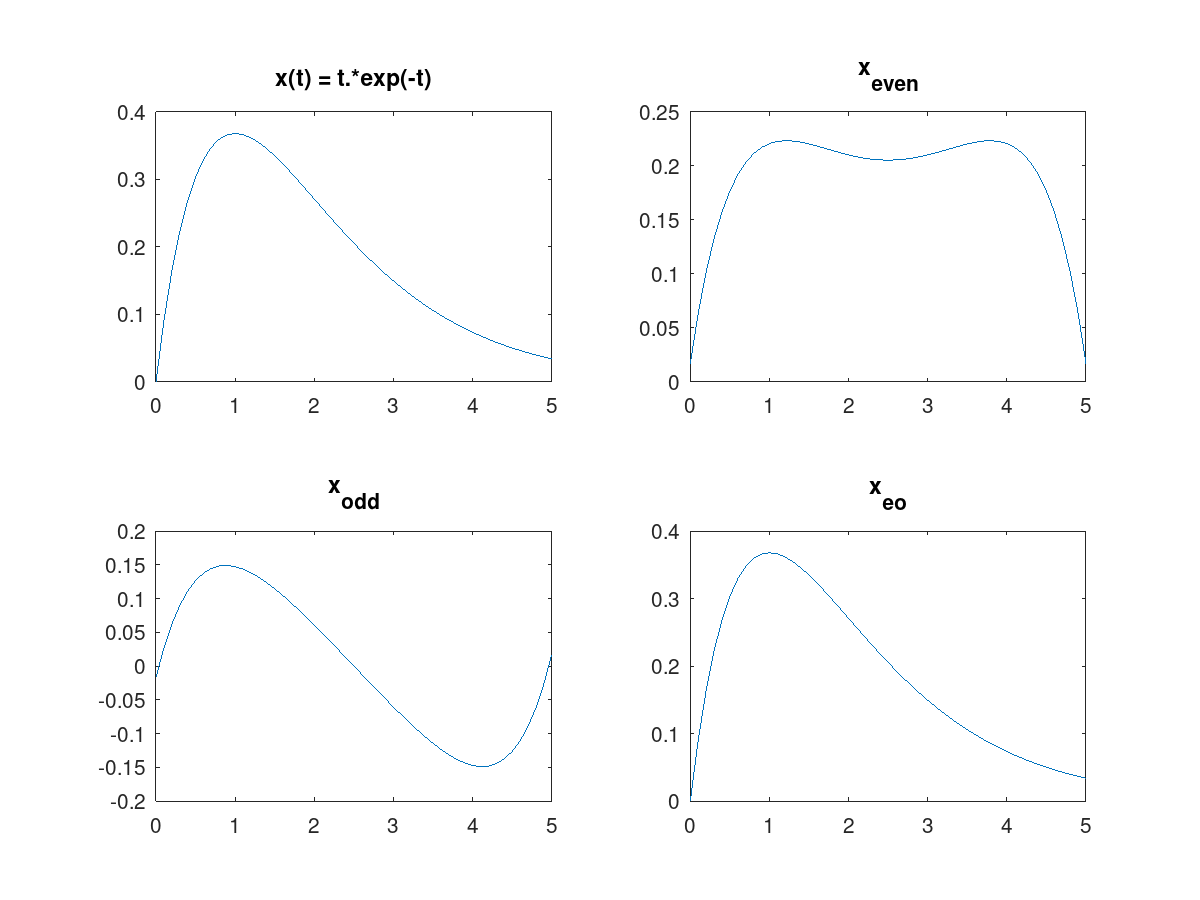
\includegraphics[width=\linewidth]{res/fig5.png}
        \caption{$x(t)$, $x_e(t)$, $x_o(t)$, $x_e(t) + x_o(t)$}
\end{figure}

\section{'Ασκηση 6}

\begin{itemize}
        \item 'Εστω το σήμα
                \[x(t) = t\cos(2\pi t), 0 \leq t \leq 5\]
                Να σχεδιάσετε τα σήματα:
        \begin{itemize}
                \item $x(t)$
                \item $x(-t)$
                \item $x(t/5)$
                \item $x(1 + 3t)$
                \item $x(-1 - 3t)$
        \end{itemize}
\end{itemize}

\begin{lstlisting}[language=octave]
        octave> t = 0:0.1:5
        octave> x1 = t.*cos(2*pi*t)
        octave> x2 = -x1
        octave> x3 = (t/5).*cos(2*pi*(t/5))
        octave> x4 = (1 + 3*t).*cos(2*pi*(1 + 3*t))
        octave> x5 = -x4
        octave> subplot(3, 2, 1)
        octave> plot(t, x1)
        octave> title("x(t)")
        octave> subplot(3, 2, 2)
        octave> plot(t, x2)
        octave> title("x(-t)")
        octave> subplot(3, 2, 3)
        octave> plot(t, x3)
        octave> title("x(t/5)")
        octave> subplot(3, 2, 4)
        octave> plot(t, x4)
        octave> title("x(1+3*t)")
        octave> subplot(3, 2, 5)
        octave> plot(t, x5)
        octave> title("x(-1-3*t)")
\end{lstlisting}

\begin{figure}[H]
        \centering
        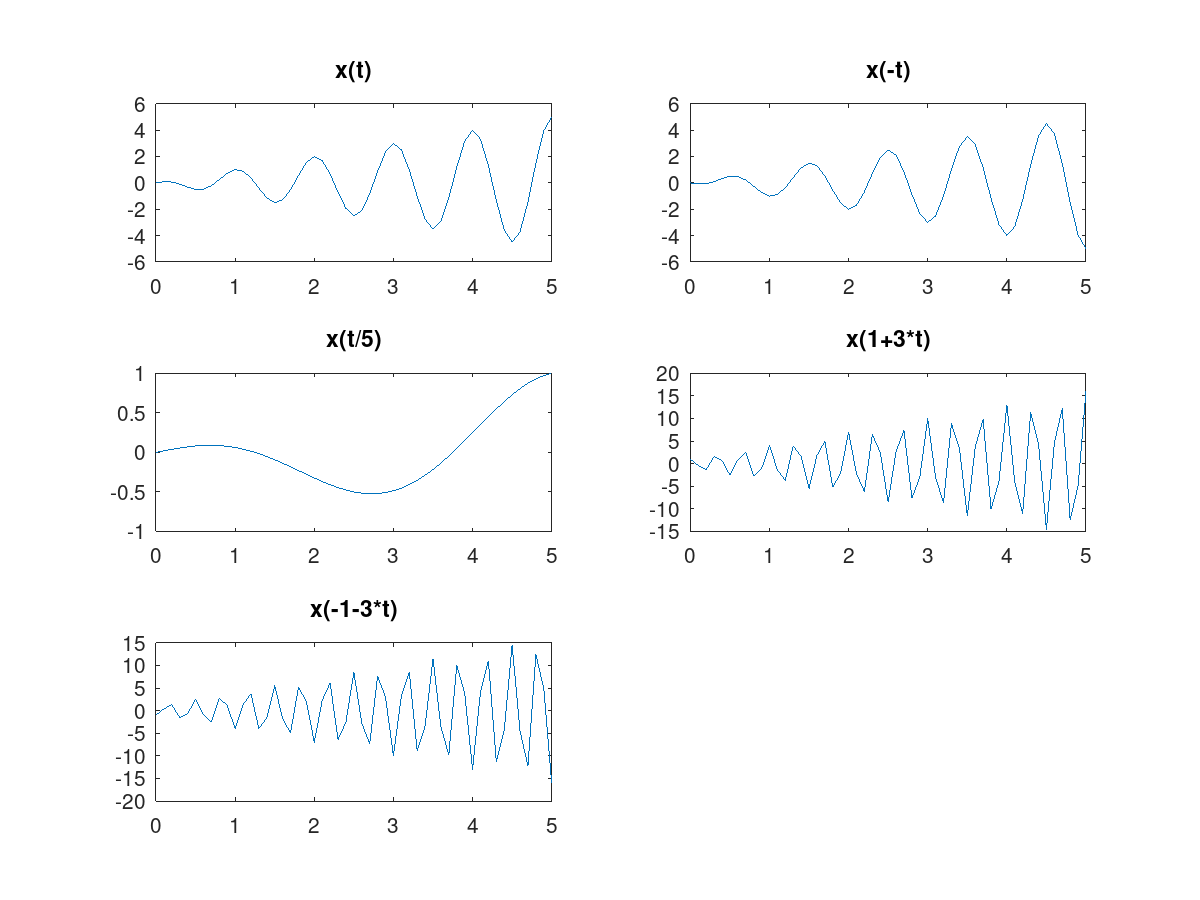
\includegraphics[width=\linewidth]{res/fig6.png}
        \caption{$x(t)$, $x(-t)$, $x(t/5)$, $x(1+3t)$, $x(-1-3t)$}
\end{figure}

\pagebreak
\section{Εργαλεία}
Τα εργαλεία που χρησιμοποιήθηκαν για την υλοποίηση αυτής της εργασίας ήτανε
τα εξής:
\begin{itemize}
        \item Περιβάλλον: GNU Octave 5.2.0
        \item Επιπλέον πακέτα:
        \begin{itemize}
                \item \lstinline{octave-forge-symbolic}
                \item \lstinline{octave-forge-signal}
        \end{itemize}
        \item Λειτουργικό σύστημα: FreeBSD 12.2
        \item Κειμενογράφος: Vim
        \item Μορφοποίηση κειμένου: \LaTeX
\end{itemize}

\end{document}
